%%%%%%%%%%%%
%% Please rename this main.tex file and the output PDF to
%% [lastname_firstname_graduationyear]
%% before submission.
%%%%%%%%%%%%

\documentclass[12pt]{caltech_thesis}
\usepackage[hyphens]{url}
\usepackage{lipsum}
\usepackage{graphicx}
\usepackage{xcolor}

%\usepackage{todonotes}

%% Tentative: newtx for better-looking Times
\usepackage[utf8]{inputenc}
\usepackage[T1]{fontenc}
\usepackage{newtxtext,newtxmath}


% Must use biblatex to produce the Published Contents and Contributions, per-chapter bibliography (if desired), etc.
\usepackage[
    backend=biber,natbib,
    %backend=natbib,
    % IMPORTANT: load a style suitable for your discipline
    style=authoryear-comp,
    uniquelist=false,
    doi=False,
    %maxalphanames=1,
    %labelalpha,
    %sorting=ynt,
    bibstyle=apj, 
]{biblatex}
\renewcommand*{\nameyeardelim}{\addspace}
%\usepackage{natbib}
%\bibliographystyle{apj}
\newcommand{\todo}[3]{{\color{#2} \emph{#1} TO DO: #3}}
\newcommand{\btmtodo}[1]{\todo{BEN}{red}{#1}}

\renewcommand{\d}[1]{\ensuremath{\operatorname{d}\!{#1}}}
\newcommand{\rsun}{{R$_\odot$}}
\newcommand{\msun}{{M$_\odot$}}
\newcommand{\kep}{{\textit Kepler}}
\newcommand{\KT}{{\textit K2}}
\newcommand{\eg}{{\it e.g.}}
\newcommand{\ie}{{\it i.e.}}
\newcommand{\spitz}{{\it Spitzer}}
\newcommand{\vsini}{{$V \sin i$}}
\newcommand{\teff}{$T_{\rm eff}$}
\newcommand{\kms}{{km\,s$^{-1}$}}
\newcommand{\gcc}{{g\,cm$^{-3}$}}
\newcommand{\rstar}{{$R_\star$}}
\newcommand{\mstar}{{$M_\star$}}
\newcommand{\rhostar}{{$\rho_\star$}}
\newcommand{\mearth}{{M$_\oplus$}}
\newcommand{\rearth}{{R$_\oplus$}}
\newcommand{\mjup}{{M$_\textrm{Jup}$}}
\newcommand{\rjup}{{R$_\textrm{Jup}$}}

\newcommand{\aj}{AJ}
\newcommand{\pasp}{PASP}
\newcommand{\apj}{ApJ}
\newcommand{\apjl}{ApJL}
\newcommand{\apjs}{ApJS}
\newcommand{\aap}{A\&A}
\newcommand{\mnras}{MNRAS}
\newcommand{\sci}{Science}
\newcommand{\nat}{Nature}


% Name of your .bib file(s)
\addbibresource{exopapers.bib}
\addbibresource{example.bib}

\begin{document}

% Do remember to remove the square bracket!
\title{Low-Mass Stars and Their Companions}
\author{Benjamin Tyler Montet}

\degreeaward{Doctor of Philosophy}                 % Degree to be awarded
\university{California Institute of Technology}    % Institution name
\address{Pasadena, California}                     % Institution address
\unilogo{caltechseal2.png}                                 % Institution logo
\copyyear{2017}  % Year (of graduation) on diploma
\defenddate{July 18, 2016}          % Date of defense

\orcid{0000-0001-7516-8308}

%% IMPORTANT: Select ONE of the rights statement below.
%\rightsstatement{All rights reserved\todo[size=\footnotesize]{Choose one from the choices in the source code!! And delete this \texttt{todo} when you're done that. :-)}}
 \rightsstatement{All rights reserved except where otherwise noted}
% \rightsstatement{Some rights reserved. This thesis is distributed under a [name license, e.g., ``Creative Commons Attribution-NonCommercial-ShareAlike License'']}

%%  If you'd like to remove the Caltech logo from your title page, simply remove the "[logo]" text from the maketitle command
\maketitle[logo]
%\maketitle

\begin{acknowledgements} 	 
   People to thank: John + group. Brendan Bowler, Justin, Luan, 
   Hogg, DFM, Ruth. 
   Ian, Dawn, Ryan, Jieun, Aaron and Jason
   Cahill department and traditions - see Sirio's.
   Antonija + Mislav, Trevor, Allison, Yi. Matt, Sirio, Gwen and Drew, Ryan.
   Committee, Patrick and Anu
   Laura
   Parents
   
\end{acknowledgements}

\begin{abstract}
   [This abstract must provide a succinct and informative condensation of your work. Candidates are welcome to prepare a lengthier abstract for inclusion in the dissertation, and provide a shorter one in the CaltechTHESIS record.]
\end{abstract}

%% Uncomment the `iknowhattodo' option to dismiss the instruction in the PDF.
%\begin{publishedcontent}%[iknowwhattodo]
% List your publications and contributions here.
%\nocite{Cahn:etal:2015}
%\end{publishedcontent}

\tableofcontents
\listoffigures
\listoftables
%\printnomenclature

\mainmatter

\chapter{Introduction}

\section{M Dwarfs: The Silent Majority}
For much of the timescale of stellar astrophysics research, to a fanatic 
of M dwarf stars their history is a story of neglect and underappreciation.
The first spectrum of an M dwarf was obtained only 100 years ago when 
\citet{Adams13} collected an observation of the M+M binary Groombridge 34.
The oldest known surviving diagram plotting stellar absolute magnitude against spectral type \citep{Russell14}, now known as a Hertsprung-Russell Diagram, includes hundreds of stars, as shown in Figure \ref{fig:HR}.
Today we know that M dwarfs make up approximately 75\% of the stars in the galaxy,
yet only $\sim$5\% of the stars included in Russell's figure are listed as
spectral type M.



\begin{figure}[hbt!]
\centering
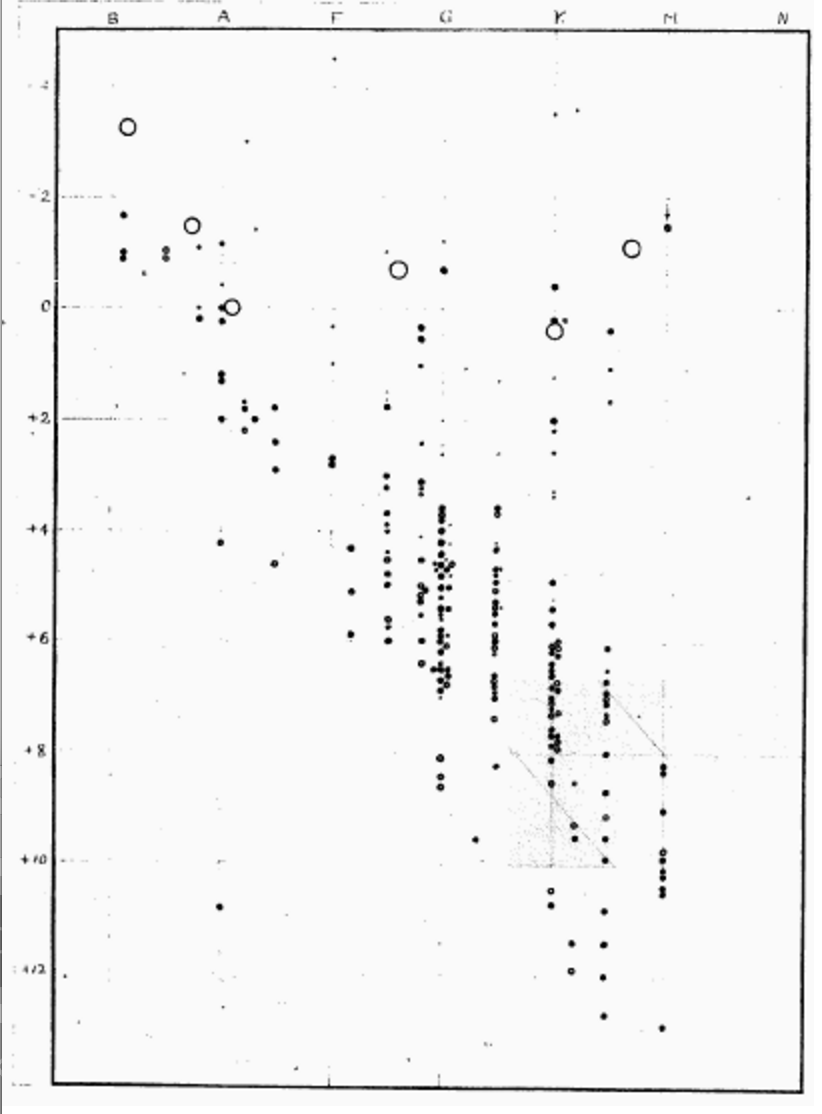
\includegraphics[width=.5\textwidth]{hr.png}
\caption[Russell's original H-R Diagram]{The original H-R diagram, as published by
\citet{Russell14}. On the $y$-axis is absolute magnitude, equivalent to the logarithm
of the star's luminosity. On the $x$-axis is stellar spectral type, which we now know
maps approximately to stellar effective temperature.}
\label{fig:HR}
\end{figure}

Russell and others hold no personal grudge against M dwarfs. The problem stems from the physics
of M dwarfs themselves, specifically the stellar mass-luminosity relation.
To show this, let us begin with the equations of stellar structure.
The first of these declares a star is in hydrostatic equilibrium:
\begin{equation}
\frac{\d P(r)}{\d r} = - \frac{ G m \rho}{r^2 },
\label{eq:hydro}
\end{equation}
where $P(r)$ is the pressure exerted on a particle at a radius $r$, $G$ is Newton's
constant, $m$ the mass enclosed inside the radius $r$, and $\rho$ the stellar density,
itself a function of radius as well.

The second equation defines mass conservation:
\begin{equation}
\frac{\d m(r)}{\d r} = 4 \pi r^2 \rho,
\end{equation}
where $\pi$ is the ratio of a circle's circumference to its diameter,
and all other variables retain their meaning from Equation \ref{eq:hydro}.

The third equation defines energy transport:
\begin{equation}
\frac{\d L(r)}{\d r} = 4 \pi r^2 \rho \epsilon,
\end{equation}
where $L$ is the energy leaving a spherical shell of radius $r$, produced by the
material in the star interior to $r$ and $\epsilon$ is the energy released per unit
mass per second inside the star.

The final equation defines the temperature gradient inside a star. 
The exact form of this equation depends on the method for which energy is transported
inside the star.
For radiative transport, the temperature gradient is
\begin{equation}
\frac{\d T}{\d r} = - \frac{3}{4ac} \frac{\bar{\kappa} \rho}{T^3} \frac{L}{4\pi r^2}.
\end{equation}
Here, $T$ is the temperature of the star at a radius $r$, $ac$ is the radiation constant multiplied by the speed of light, also equal to four times the Stefan-Boltzmann
constant, and $\bar{\kappa}$ the mean opacity of the material.

Very low-mass stars are fully convective, not radiative, and therefore follow
a different limit:
\begin{equation}
\frac{\d T}{\d r} =  \bigg( 1 - \frac{1}{\gamma}\bigg)\frac{T}{P}\frac{\d P(r)}{\d r},
\end{equation}
where $\gamma$ is the adiabatic index, and is $5/3$ for a monatomic ideal gas,
and all other terms retain their previous meaning.

Let us consider two other proportionalities. First, we assume that the energy generation rate
inside a star is a function of its temperature and density:
\begin{equation}
\epsilon = \epsilon_0 \rho T^\nu
\end{equation}
where $\nu$ depends on the particular fusion pathway that is dominant in the core of
the star.
Second, we assume that the ideal gas law holds:
\begin{equation}
P \propto \rho T.
\end{equation}

With these six equations, we can develop a series of homology relations. We can create
a series of five linear equations with five unknown parameters: $\log T$, $\log P$, 
$\log R$, $\log \rho$, and $\log M$.
Ignoring constant terms and considering only the adiabatic case (as for fully 
convective stars),
\begin{align}
\log P &= 2 \log M - 4 \log R \nonumber \\
\log \rho &= \log M - 3 \log R \nonumber \\
\log P &= \gamma \log \rho \\
\log T &= \bigg(\frac{\gamma - 1}{\gamma}\bigg) \log P \nonumber \\
\log L &= \log \rho + \nu \log T + \log M \nonumber.
\end{align}
We can rearrange these to solve for $\log M$, finding
\begin{equation}
\log R = \bigg(\frac{2-\gamma}{4 - 3\gamma}\bigg) \log M,
\end{equation}
which we can then insert into the final equation in Equation 1.8.
This manipulation yields
\begin{equation}
\log L = \bigg(\frac{2(\nu + 1) - \gamma(2\nu + 3)}{4 - 3\gamma}\bigg) \log M,
\end{equation}
which if we consider the case where we have an ideal, fully ionized gas so that $\gamma = 5/3$ and energy generation dominated by the p-p chain so that $\nu = 4$, we find
\begin{equation}
\log L \approx 8.33 \log M
\end{equation}
or $L \propto M^{8.33}$! Thus, if we decrease the mass of a fully convective star by a factor of two, 
we also decrease its luminosity by a factor of 320!\footnote{The same manipulation,
considering the case of radiative transport, leads to the relation $L~\propto~M^{5.5}$,
similar to what is observed for Sun-like stars.} 

Even worse for optical observing,
the peak of the SED of a typical 3,000 K M dwarf peaks at 1 micron, well into the infrared, making them even fainter in the optical.
Even though M dwarfs make up 70\% of the nearest stars, with 250 of them located within
10 pc of the Sun \citep[e.g.][]{Henry06}, there are no M dwarfs visible to the naked 
eye.
The brighest, HIP\,105090, is only $3.95 \pm 0.01$ pc from the Sun, yet has an apparent V-band magnitude of 6.76 \citep{vanLeeuwen07}.
With so many bright solar-type stars in the solar neighborhood, it is easy to understand why M dwarfs have been and often continue to be overlooked in planet search
surveys. 

\section{Radial Velocity Planet Searches}
The first radial velocity (RV) planet searches focused almost exclusively on Sunlike
(FGK) stars. 
There are two biases that make this a reasonable choice of star. 
First, 

FGK are good
found a bunch of new planets
why change?

Slowly moved into searches for planets around other types of stars
John's subgiants
M dwarf searches---CPS and HARPS
Didn't find so many

RV limitations: large planets, close in.
Can't find very small planets, or very distant ones
what's the best place to search? Mike Bottom's paper.

Planets in wide orbits: motivate TRENDS survey.

\section{Transiting Planet Searches}
\subsection{The Importance of Transiting Planets}
If a planetary system is aligned in such a way that the planets pass between our
viewing position in the solar system and the star itself, they will appear to pass
across (or transit) the stellar disk during their orbit.
We can not resolve the surface of the star in order to image the transit itself, but
we can still detect it. 
During the transit, a portion of the stellar disk is blocked, decreasing the observed
flux from the star. 
The size of this decrement, termed $\delta$, corresponds to the fractional area of the star's disk blocked by the planet:
\begin{equation}
\delta = \bigg(\frac{R_p}{R_*}\bigg)^2.
\end{equation}
Again, we find that we must understand the star's parameters (in this case, the radius)
in order to understand the planetary parameters.

Detecting planets with the transit method is more limited relative to the RV method:
only a small fraction of all planets will be directly detectable. 
Any planets not in nearly edge-on orbits will be missed in a transit search.
In addition, transit photometry provides precise information about the location 
of a planet, but only at one point of its orbit.
Even in cases where information about the eccentricity can be inferred from the
transit itself \citep{Dawson12a}, there is still a degeneracy
between the eccentricity and argument of periastron which can not be broken without
additional information.

On the other hand, there are a few key advantages in transit searches relative to 
RV surveys. 
Transit searches can target many more stars than RV surveys. 
To a first order approximation, transits are achromatic, with the depth of the transit
approximately equal at all wavelengths, so transits can be detected through broadband
photometry.
As RV surveys require high-resolution spectroscopy, they require comparatively brighter
stars; transit searches can target significantly fainter stars, opening up the search
for planets to many more M dwarfs.
Similarly, as spectral features are no longer required, transit surveys can target 
rapidly rotating massive stars without convective outer layers and narrow spectral lines.

Transit surveys also allow for a more direct determination of the planetary physical 
properties. 
In RV searches, only a minimum mass
for the detected planet, $m \sin i$, can be determined. 
Although the planet mass distribution and geometrical bias both favor large
(close to edge-on) inclinations \citep{Ho11}, individual objects have unknown inclinations
so the absolute masses of the RV planets cannot be determined.
In transit searches, however, the direct observable is the transit depth, which depends
directly on the size of the planet: for a sufficiently precise measurement of the stellar
radius and transit parameters, any precision on the planet radius can be achieved without
a geometric bias.

Perhaps most significantly, transit searches allow us to probe atmospheres of
other planets.
Planetary atmospheres, Earth's included, are optically thick at some wavelengths and
optically thin at others. 
In the context of the Earth, this makes some wavelengths more amenable for astronomical
observations than others, as the atmosphere only interacts with photons of certain
wavelengths.
The same is true for planets around other stars: at same wavelengths their atmospheres
are transparent to radiation from their host stars, while at other wavelengths
the atmospheres absorb light.
By observing a transit at a wavelength at which the atmosphere is optically thick, the
size of the planet inferred is the size of the planet, including its atmosphere.
Alternatively, by observing at a wavelength at which the wavelength is optically thin,
we measure only the size of the planet itself, not its atmosphere \citep[e.g.][]{Knutson11, Knutson14}. 
Such an analysis, termed \textit{transmission spectroscopy}, is impossible in traditional RV searches for planets.

To fully understand the atmosphere measured during transmission spectroscopy observations,
we want to understand the mass (and therefore the density) of the transiting planet as
well.
If the transiting planet is massive and the star a good RV target (bright and not 
rapidly-rotating), RVs can be used to meaure a mass. 
Since the planet is known to be transiting, it must have $i \approx \pi/2$, so that
$\sin i \approx 1$. 
Unfortunately, the vast majority of transiting planets are too faint to make ideal
RV targets.
In these cases, we would like to have an alternative method to measure masses.

When multiple planets orbit the same star, they gravitationally perturb each other
during close encounters along their orbit.
Transit photometry provides precise information about the location of a planet on its 
orbit at the moment of transit, especially the times at which the transits
begin and end.
In \kep\ data, it is not uncommon to be able to measure individual times of transit to a
precision of five minutes or better, with the exact precision a function of the 
planet size (which affects the size of each individual transit) and orbital period
(which affects the speed at which a planet orbits its host star, assuming a 
circular orbit).
Perturbations from other planets can be significantly larger than the transit timing
precision, leading to transit timing variations (TTVs). 
For a hypothetical distant observer detecting transits in our solar system, the
presence of Jupiter could be inferred from TTVs on the inner planets: 
Jupiter induces TTVs of 10 minutes on Venus and Earth and 100 minutes on Mars
\citep{Agol05, Holman05}.

\kep\ enabled the first detections of TTVs. 
Timing variations have been used to confirm the planetary nature of apparent transiting
planet signals in \kep\ \citep{Holman10, Rowe14}.
They have also enabled the detection of non-transiting planets perturbing transiting
planets \citep[e.g.][]{Ballard11, Nesvorny13}, as well as measurements of the eccentricity 
distribution of transiting planets \citep{Hadden14}.
Observations of TTVs enable a direct measurement of the mass ratio between the
perturbing planet and the host star \citep{Agol05, LithwickWu12},
again enabling us to understand the mass of the transiting planet at the level 
at which we understand the mass of the host star.
 


\subsection{History of Transit Searches}
The first transiting planet detected was a giant planet orbiting HD\,209458 
\btmtodo{Cite: Charbonneau, Henry}. 
This planet, a hot Jupiter, has a radius of $1.14 \pm 0.06$ \rsun\ and an orbital 
period of 3.52 days.
The planet was already known to exist from RV surveys, and had a measured $m \sin i$.
Detection of the transit provided a measurement of the inclination, enabling a 
direct measurement of the mass; the transit detection made it the first planet outside our solar system with a directly measured mass and radius.

Shortly after came the first discovery of a planet via transit, OGLE-TR-56b \btmtodo{Cite} from the Optical Gravitational Lensing Experiment (OGLE) mission.
The primary goal of OGLE is to detect dark matter through microlensing, but it has also discovered 
many planets via microlensing \btmtodo{Cite}.
Microlensing surveys are also ideal for the discovery of transiting planets, as 
I discuss in Chapter~\ref{chap:wfirst}.

Transit surveys discovered 45 more planets between these initial discoveries and 2009, largely through dedicated surveys such as WASP \btmtodo{CITE}, HAT \btmtodo{CITE}, and
CoRoT \btmtodo{CITE}.
These planets were largely giant planets in short periods, similar to the early hot Jupiters
detected by RV surveys. 

In 2009, the \kep\ mission \citep{Borucki10} was launched and began taking data.
At this point, the exoplanet community had discovered 45 planets via the transit
method.
The precision of \kep\ was significantly better than any previous mission, allowing
20 part per million (ppm) photometry over six hours of observation on 12th magnitude
stars. 
It also had a large field of view, staring at 100 square degrees of the northern sky.
Every 30 minutes, the telescope recorded photometry of approximately 180,000 stars in a
search for periodic transits caused by small planets.

Any combination of words less strong than ``tremendous success'' would significantly undersell the data from \kep.
The mission has discovered more than 4,700 planet candidates to date, with more than 
2,300 of these being confirmed via other methods or statistically validated as planets
to a high confidence \btmtodo{Cite Tim's recent paper, and the typical KOI papers}.
Most of the stars targeted by the mission are Sunlike FGK dwarfs, so most of the discovered
planets transit Sunlike FGK dwarfs.
However, there were approximately 5,000 M dwarfs in the original \kep\ target list, around
which more than 100 planets have been discovered.
These include planets as small as Mars \citep{KOI961} and a planet as large as Jupiter
\citep{Johnson11c}.
These planets are located in different environments, with some located in single systems
and others tightly packed in resonant chains with low eccentricities and mutual inclinations
\citep{Swift13, Ballard16}.
\citet{Morton14} show that these planets are predominantly small, rocky planets in short
periods around their host stars.

Many papers have focused on the planets detected around M dwarfs, but there are ``only'' 100
of them from the \kep\ mission around 5000 stars. As \kep\ is largely a magnitude-limited
survey, the majority of the M dwarfs surveyed are early M0 and M1 dwarfs. 
Only 300 stars had an M2 or later spectral type in the original mission, and only 30 had
an M4 or later spectral type.

The \KT\ mission is providing an opportunity to rectify this oversight.
With the failure of two reaction wheels on the \kep\ spacecraft in 2013, the telescope
was left unable to point at the original \kep\ field, ending the primary mission.
The scientific and technical staff behind \kep\ then designed, with community input,
a mission called \KT. 
In this mission, the telescope uses the remaining two reaction wheels to point the telescope
along the ecliptic plane, while the third axis is approximately balanced by solar radiation
pressure.
The telescope then rolls about its axis at approximately 1 arcsec hour$^{-1}$, which 
the telescope corrects by periodically firing its thrusters in the opposite direction
of the roll.
In the \KT\ mission, the telescope is able to point at fields in the ecliptic plane for
approximately 75 days at a time.
By the end of the \KT\ mission, the telescope will point at approximately 20 fields
covering the ecliptic plane.

\KT\ is extremely important for the study of M dwarfs.
Different fields in the ecliptic point towards or well out of the galactic plane.
The typical G dwarf observed in the \kep\ mission in 300 pc from the Earth, so changes
in galactic latitude vastly affect the number of bright FGK dwarfs observable.
The typical M dwarf, however, is 50 pc from the Earth, so even pointing directly out of the
galactic plane does not affect the stellar density by more than a factor of two, making 
tens of thousands of M dwarfs observable during the mission. 
\KT\ provides an opportunity to revolutionize our understanding of planets around M dwarfs,
if we can confirm planets and characterize their host stars with data from the telescope.

\section{Understanding M Dwarfs}
One of the other downsides of studying companions to M dwarfs is the difficulty 
in inferring stellar parameters.
For both RV-detected and transiting planets, the measured quantity of interest 
(the Doppler amplitude and transit depth) are a function of both planetary and stellar
parameters. 
In both cases, we are only able to understand the planet if we understand its host star:
precision planetary astronomy requires precision stellar astronomy.

For solar-type stars, we are able to infer stellar parameters at the few percent level,
even without a measurement of the star's luminosity through a parallax measurement
\btmtodo{Cite this claim}.
This is largely possible due to an excellent calibration source located 1 AU away from the 
Earth.
For M dwarfs, 
\btmtodo{No calibrator, Physics is more complicated, photons are more scarce.}

Attempts to understand M dwarf atmospheres and interiors typically depend on empirical 
relations between photometric or spectroscopic parameters, calibrated to a few stars
with known properties.
These calibrators tend to be eclipsing binaries with directly measured masses and radii \btmtodo{Cite 
examples} or single, nearby stars with interferometrically measured radii \btmtodo{Cite Tabby}.
For example, \btmtodo{Delfosse}

\btmtodo{Where are we as a field in M dwarf params? Much closer than 5 years ago
but still not great}

The problem is even worse when we consider young M dwarfs.
\btmtodo{Grab words from proposals here.}

For very young stars, we can measure their masses by observing the kinematics of
the disk of gas and dust surrounding the star \citep{Czekala15, Czekala16}.
These disks dissipate within the first ten million years of the star's life, decreasing the opportunity to measure directly the masses of stars with ages larger than 10 million years but not yet onto the main sequence. 
This is especially true for M dwarfs, which are faint, so harder to observe, and also 
form in binaries less often than their higher mass counterparts \citep{Fischer92, Shan15}.
Fewer than 20 pre-main sequence (PMS) M dwarfs in binary systems have had dynamical masses measured to a
precision of 25\% or better through astrometric monitoring \citep{Dupuy14}.
The vast majority of these systems are younger than 10 Myr.
In the range 10-100 Myr, for a given luminosity and age, different stellar models predict different stellar masses, some with discrepancies as large as 50\% \citep{Hillenbrand04,Schlieder14}.
Measuring stellar masses of astrometric M+M binaries in young moving groups with known 
ages provides a first, needed test of these models in order to constrain evolutionary models.

\section{Brown Dwarfs}
Brown dwarfs are typically the most massive of substellar objects. 
The exact definition of what qualifies as a brown dwarf is a matter of dispute.
Often, especially among observers, the boundary is based on the mass of the object.
Objects larger than 13 \mjup, in which deuterium burning can occur in their core for
at least a small fraction of their lifetime, are considered brown dwarfs.
Objects for which conditions in the core are sufficient for hydrogen burning, at approximately 
72 \mjup, are considered stars \citep{Zuckerman00}.
This definition is the official definition of a brown dwarf from the International
Astronomical Union.

However, recent evidence suggests two formation pathways for 13-72 \mjup\ objects
\citep{Bayliss16}. 
On the low-mass end, there is a population of transiting brown dwarfs in short orbital
periods which may have formed via core accretion, like planets.
On the high-mass end, there is a population of transiting brown dwarfs in wider orbital
periods which may have formed via gravitational collapse, like other high mass-ratio
eclipsing binaries.
In the middle, there is a ``brown dwarf desert,'' with a paucity of 30-50 \mjup\ objects in
binary systems.
Some, especially theorists, have suggested a definition of brown dwarfs based on their
formation, with all objects formed via core accretion called planets and all objects
formed via gravitaitonal collapse (but below the hydrogen burning limit) brown dwarfs
\citep[e.g.][]{Chabrier14}.
In this thesis, I will follow the IAU definition of a brown dwarf, noting that none of the
claims presented within would be significantly affected by following the althernative
definition.

Many of the problems for M dwarfs outlined in this introduction are even worse for
brown dwarfs.
Without active hydrogen burning, they can be significantly fainter than M dwarfs.
They cool and collapse in time, meaning their luminosity is continuously decreasing:
they can be considered to be effectively PMS objects for longer than the age of the 
universe \citep{Burrows01}.
Understanding the physical parameters of an individual brown dwarf requires an assessment of its age as well.

Broadly speaking, there are two classes of brown dwarfs.
Approximately two thousand brown dwarfs have been detected as single objects in the sky,
largely through IR surveys like 2MASS and WISE \citep[e.g.][]{Kirkpatrick99, Kirkpatrick11}.
For these objects, we are able to study their atmospheric properties in detail: we can 
infer the presence of clouds, measure a rotation period, or obtain a spectrum and measure
spectroscopic properties like the surface gravity or effective temperature \citep[e.g.][]{Faherty14, Filippazzo15}. 

What we are not able to do is measure masses and radii for these single objects.
There are only two eclipsing brown dwarf systems known, one in the $\sim 1$ Myr old Orion
Nebula cluster and one in the $\sim 10$ Myr old Upper Scorpius young moving group
\citep{Stassun06, David16}.
As both of these are extremely young, they are not representative of the field brown dwarf
population so do not provide useful benchmark comparisons.
Among older systems, we know of approximately ten systems with a brown dwarf transiting a main-sequence star, as I will describe in Chapter \ref{chap:lhsspitz}.
The vast majority of these systems include a brown dwarf in a short period orbiting
close enough so that the energy from stellar irradiation is significantly larger than
the emitted heat from the cooling of the brown dwarf, irradiating and possibly inflating
the atmosphere of the brown dwarf.
In these cases, the brown dwarfs will again appear significantly different from the field
brown dwarf population, eliminating the possibility that these could be used as benchmark
objects to calibrate brown dwarf masses and radii.


We would ideally want a transiting brown dwarf receiving a low level of irradiation,
so we can measure its mass and radius.
We would also want this brown dwarf to be nearby so we can measure its atmosphere to
compare to the field brown dwarf population, providing a key test of brown dwarf
evolutionary models.

If we want a transiting object that is nearby and not highly irradiated by its companion,
an ideal place to search is around M dwarfs. 
As stated previously, M dwarfs in transit searches are typically much closer than 
higher mass stars, as transit surveys tend to select magnitude-limited samples and
M dwarfs are intrinsically faint. 
Moreover, their low luminosities mean a companion at a given separation will receive
significantly less irradiation than the same companion around a higher mass star,
so that relatively short periods can allow for non-irradiated companions.

The equilibrium temperature for an object with albedo $a$ at a given separation, $r$, from a 
stellar companion with radius \rstar, is
\begin{equation}
T_{\textrm{eq}} = T_\star (1-a)^{1/4} \sqrt{\frac{R_\star}{2r}}.
\end{equation}
A 65 \mjup\ brown dwarf has a temperature of 1100 Kelvin even at the age of 
the universe \citep{Saumon08}. 
Such a brown dwarf around an M dwarf would be expected to have an albedo of
0.07 \citep{Marley99}.
For this brown dwarf to have an equilibrium temperature of 1100 Kelvin orbiting a
3000 Kelvin M dwarf, it would need to orbit at only 3.7 stellar radii, or approximately
0.01 Astronomical Units (AU), corresponding to an orbital period of approximately one day.
Therefore, even M dwarf-brown dwarf binaries with few day periods can provide useful 
comparisons to the field brown dwarf population.
Of course, this brief calculation ignores the possible effects of interactions between
the magnetic fields of the two objects. These could play a significant role, as 
observations of aurorae on brown dwarfs suggest they can have magnetic fields exceeding
2000 Gauss \citep{Hallinan15}






\section{Goals of this Thesis} 

\btmtodo{See Drew's thesis for tips on formatting previous papers section}







\chapter{This is the Second Chapter}


\begin{figure}[hbt!]
\centering

\includegraphics[width=.3\textwidth]{caltech.png}
\caption[Example Figure]{This is a figure}
\label{fig:logo}
\end{figure}

\subsection{This is a subsection}

\begin{table}[hbt!]
\centering
\begin{tabular}{ll}
\hline
Area & Count\\
\hline
North & 100\\
South & 200\\
East & 80\\
West & 140\\
\hline
\end{tabular}
\caption[Table]{This is a table}
\label{tab:sample}
\end{table}



\btmtodo{This is the Dynamical Masses TTV paper}


\chapter{This is the Third Chapter}



\btmtodo{This is TRENDS IV}

\chapter{This is the Fourth Chapter}

\btmtodo{This is LHS Part 1}
\chapter{This is the Fifth Chapter}

\btmtodo{This is LHS Part II}
\label{chap:lhsspitz}

\chapter{This is the Sixth Chapter}

\btmtodo{This is the M+M binary work}

\chapter{This is the Seventh Chapter}

\btmtodo{This is the K2 planet catalog}

\chapter{This is the Eighth Chapter}
\label{chap:wfirst}

\btmtodo{This is WFIRST}

\chapter{This is the Ninth Chapter}

\btmtodo{This is the summary and future directions}

\printbibliography[heading=bibintoc]
%\bibliography{exopapers}

%\appendix

%\chapter{Questionnaire}
%\chapter{Consent Form}

%\printindex

%\theendnotes

%% Pocket materials at the VERY END of thesis
%\pocketmaterial
%\extrachapter{Pocket Material: Map of Case Study Solar Systems} 


\end{document}

